\chapter{Introducción}
\label{capitulo1}
\lhead{Capítulo 1. \emph{Introducción}}

En los últimos años se han logrado avances importantes en el área de navegación y exploración con robots móviles, lo que ha permitido ampliar las aplicaciones de estos en espacios áereos, terrestres y acuáticos en diversas disciplinas, facilitando la extracción de información de estos entornos en lugares de difícil acceso.

En este sentido el Grupo de Investigación y Desarrollo en Mecatrónica de la USB \textit{(GIDM)} ha venido desarrollando un conjunto de proyectos relacionados con los sistemas de navegación de robots autónomos y de operación remota de estos desde el año 2013, donde el área de odometría y SLAM se ha venido trabajando con profundo interés por ser fundamental en la recopilación de información de diferentes ambientes y por abrir la puerta a la automatización de la exploración y navegación de vehículos autónomos.

\section{Antecedentes}

En el \textit{GIDM} se han realizado grandes avances en el desarrollo de equipos y plataformas robóticas para actividades de investigación, exploración e inspección de ambientes no estructurados. Usualmente cuando se opera en este tipo de ambientes, en busca de realizar exploraciones mas eficientes y a mayor escala, se emplean vehículos operados remotamente \textit{ROV} (del inglés: Remotely Operated Vehicles) equipados con cámaras de vídeo. O bien, para el caso de aplicaciones subacuáticas también se suelen utilizar vehículos autónomos submarinos \textit{AUV} (del inglés: Automated Underwater Vehicles), mientras que para exploraciones aéreas se hace uso de vehículos aéreos no tripulados UAV (del ingles: Unmanned Aerial Vehicle).

En este sentido, en el año \textit{Certad, N.} \cite{novel} propuso en el 2013 como proyecto de maestría, un algoritmo de localización y mapeo simultáneo ppara un vehículo terrestre de locomoción diferencial instrumentado con sensores exteroceptivos, realimentado por odometría, el cual utilizó Webots como herramienta de simulación y fue implementado utlizando Matlab.


\begin{figure}[H]
	\centering
	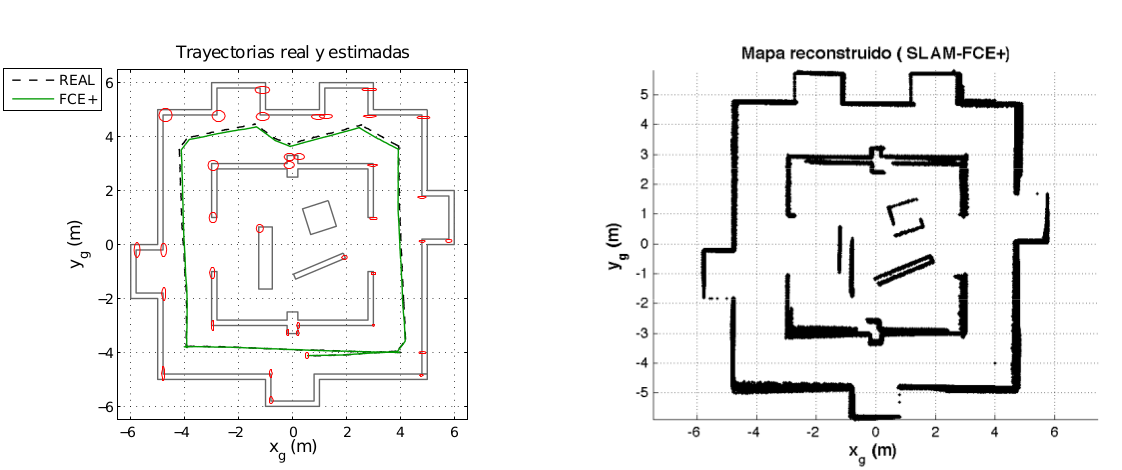
\includegraphics[width=0.7\textwidth]{Antecedentes/Certad}
	\caption{Resultados de trayectoria y reconstrucción de mapas obtenidos en \cite{novel}}
	\label{imagen:Antecedentes/Certad}
\end{figure}





En el 2017, \textit{Gonzáles M.} \cite{manuel} desarrolló un sistema de reconstrucción de modelos de ambiente utiliznado un sensor de Detección y Localización por Láser (LIDAR, del inglés: Laser Imaging Detection and Ranging). Esta implementación se realizó utilizando ROS como núcleo de control y procesamiento de datos y \textit{Cartographer} como herramienta de manejo de la localización y mapeo del prototipo empleado. Los modelos reconstruidos como el presentado en la figura \ref{imagen:Antecedentes/octomaps} se realizaron utilizando estructuras probabilísticas de ocupación llamadas \textit{octomaps}, las cuales permitieron la disminución del uso de recursos de memoria en la reconstrucción de grandes entornos.


\begin{figure}[H]
	\centering
	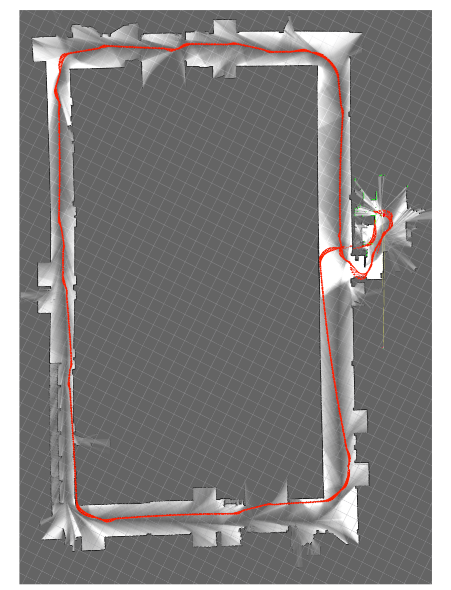
\includegraphics[width=0.3\textwidth]{Antecedentes/mapa2D}
	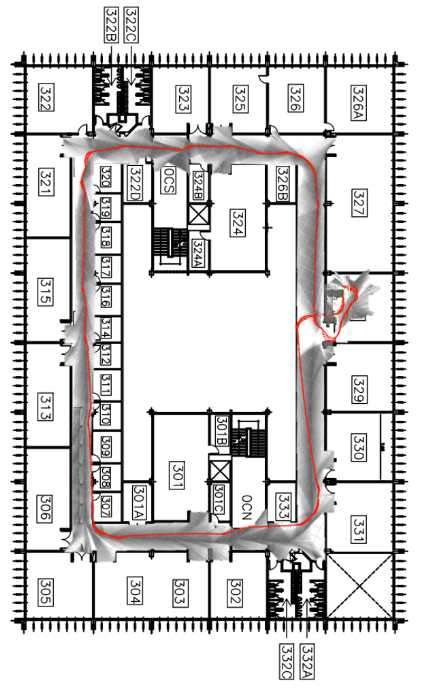
\includegraphics[width=0.3\textwidth]{Antecedentes/mapa2DReal}
	\caption{Resultados de trayectoria y reconstrucción de mapas obtenidos en \cite{manuel}. A la izquierda se presenta el mapa original obtenido y a la derecha se presenta superpuesto al diagrama del edificio real.}
	\label{imagen:Antecedentes/mapa2D}
\end{figure}


\begin{figure}[H]
	\centering
	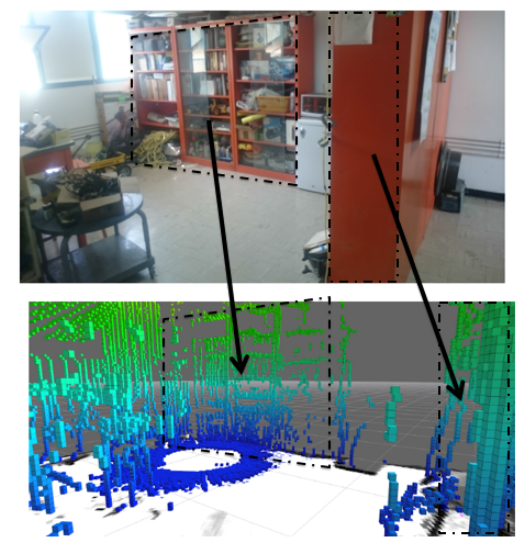
\includegraphics[width=0.7\textwidth]{Antecedentes/Octomaps}
	\caption{Reconstrucción en tres dimensiones utilizando octomaps obtenidos
		en  \cite{manuel}}
	\label{imagen:Antecedentes/octomaps}
\end{figure}

 En este sentido, se tienen proyectos como el presentado por \textit{Danilo, D.} \cite{danilo}, cuyo proyecto de grado consistió en el desarrollo en un sistema de operación remota para un prototipo de robot submarino (\textit{Poseibot}), con la finalidad de implementarlo en tareas de exploración. Con objetivos similares, \textit{Said, A.} \cite{said} basó su proyecto de grado en la instrumentación y control de un robot cuadricóptero volador(\textit{UAV}) diseñado y fabricado también como parte de dicho proyecto. 

Adicional a los dos prototipos antes mencionados, en el \textit{GIDM} se cuentan con otras plataformas móviles como \textit{Roomba}, \textit{AmigoBot}, y un vehículo submarino OpenROV\footnote{ \url{https://www.openrov.com/products/openrov28/}}, el cual es un robot maniobrado remotamente de baja envergadura, diseñado especialmente operaciones de exploración y está dotado, entre otras cosas, con una cámara de video HD y una unidad de medición inercial.

\begin{figure}[H]
	\centering
	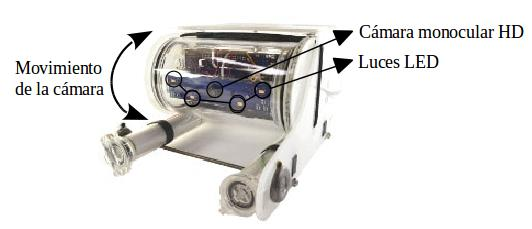
\includegraphics[width=0.7\textwidth]{openrov}
	\caption{Robot móvil OpenROV}
	\label{imagen:openrov}
\end{figure}

Si bien se cuenta con un conjunto de plataformas robóticas adaptadas para tareas de exploración, hasta el momento los sistemas de navegación y mapeo empleados han estado basados en GPS y telémetro láser, pero aún no se ha concluido el desarrollo de sistemas basados en visión que permitan la navegación y mapeo. La presente investigación es la primera en abordar la tarea de la reconstrucción de la superficie recorrida haciendo uso únicamente de una cámara de vídeo, sensor presente en todas las plataformas robóticas antes mencionados.

\section{Justificación y planteamiento del problema}

El Grupo de Investigación y Desarrollo en Mecatrónica de la USB ha venido desarrollando un conjunto de proyectos relacionados con los sistemas de navegación de robots autónomos y de operación remota de estos. Actualmente cuentan con un vehículo submarino OpenROV 2.8 de operación remota (ROUV, por sus siglas en inglas - Remotely Operated Underwater Vehicle) el cual posee una IMU y tiene la capacidad de transmitir videos en alta definición. Es por ello que los trabajos más recientes de este grupo han estado enfocados al área de visión por computadora con la finalidad de mejorar el desempeño y las capacidades de los sistemas de control de vehículos como el OpenROV 2.8, y para realizar exploración submarina como reconstrucciones y muestreos de arrecifes, embarcaciones hundidas y fauna submarina. Entre estos trabajos se encuentra el proyecto de grado de Fabio Morales, en el cual se implementó un sistema de odometría visual para resolver el problema de SLAM en robots submarinos basado en una cámara monocular, y el proyecto de grado de  Armando Longart, en el cual se desarrollaron módulos de procesamiento de imágenes y video para aplicaciones subacuáticas.

Dichos trabajos permiten la posibilidad de ser integrados  y optimizados en un nuevo sistema de SLAM visual más robusto, y que además permita ser extendido para robots en diferentes entornos, automatizando la generación de las operaciones de mapeo y localización del vehículo.

\section{Objetivos}

\subsection{Objetivo General}

Analizar e implementar un sistema automatizado que permita la localización de un robot terrestre, aéreo o submarino, a través de la información capturada por una cámara monucular y una unidad de medición inercial, además de realizar un mapa de su entorno.

\subsection{Objetivos Específicos}

\begin{itemize}
	\item  Revisar la localización y mapeo simultáneo en robots móviles (aéreos, terrestres y submarinos) basados en cámara.
	\item Revisar los métodos de procesamiento de imágenes convenientes para los algoritmos de SLAM visual en función del entorno del robot móvil.
	\item Implementar un sistema de SLAM visual.
	\item Generar la posición, trayectoria del robot móvil y  un mapa 3D aproximado de su entorno.
\end{itemize}

\section{Estructura del trabajo}

Luego de presentar el planteamiento del problema y la descripción del proyecto, el presente trabajo se encuentra estructurado en 5 capítulos, donde se explica todo el desarrollo realizado y está organizado de la siguiente manera:

En el \textit{\textbf{Capítulo 2}} se presenta una revisión del estado del arte sobre los algoritmos de generación de mosaico, en el cual se exponen los trabajos recientes y avances importantes en esta área de investigación. Al mismo tiempo, se describen los módulos principales que componen este tipo de sistemas. Luego, en base a los algoritmos y técnicas estudiadas, se propone un esquema para un sistemas de generación de mosaico. Para finalizar, se presenta la librería de procesamiento de imágenes que se planteó utilizar para la implementación de los algoritmos propuestos.

El \textit{\textbf{Capítulo 3}} inicia una revisión teórica en la cual se describe el funcionamiento de los algoritmos detectores, descriptores y emparejadores de características; y posteriormente se presentan resultados de pruebas comparativas entre los mas usados para este tipo de aplicaciones. 

El módulo encargado de la alineación de imágenes en el mosaico, es descrito en el \textit{\textbf{Capítulo 4}}. Al igual que el capítulo anterior, se presenta una revisión teórica de los conceptos necesarios para su implementación. Luego, se introduce el modelo de submosaicos, y la implementación de un conjunto de correcciones geométricas sobre este nuevo modelo. Finalmente se muestran los resultados de los algoritmos aplicados en esta sección, seguidos de sus respectivos análisis.

En el \textit{\textbf{Capítulo 5}} se describe el módulo final del sistema, en donde se explica el funcionamiento de los algoritmos que corrigen visualmente el mosaico definitivo. De igual forma se muestran los resultados de su implementación, seguidos de una conclusión final sobre estos.

Finalmente, en el \textit{\textbf{Capítulo 6}} se presentan las conclusiones derivadas del proyecto, además de propuestas sobre recomendaciones y posibles implementaciones que pueden aportar mejoras y/o permitir la continuación del desarrollo de investigación aquí descrito.
